\chapter{Table of contents}
\label{ch:kap1}

\section{Document Structure} 
\label{sec:struktur}

The report is structured like this:

In chap. ~\ref{ch:kap1} Introduction

In chap. ~\ref{ch:kap2} Inspiration

In chap. ~\ref{ch:kap3} Concept

In chap. ~\ref{ch:kap4} Design

In chap. ~\ref{ch:kap5} Programming

In chap. ~\ref{ch:kap6} Playtesting

In chap. ~\ref{ch:kap7} Pre-Production

In chap. ~\ref{ch:kap8} Production

In chap. ~\ref{ch:kap9} Project Management

In chap. ~\ref{ch:kap10} Group Dynamics

In chap. ~\ref{ch:kap11} Conclusion


\newpage

\section{Project Description}
\label{sec:Description}
When it comes to making a game, it is a challenge to make something original and unique. This especially since it feels like everything has already been done. That was one of our bigest objectives when developing the idea behind the game we call "CardLords High School". The challenge is making a 2D material such as cardboard work in a 3D environment, therfore this projects focus lies on making a what we refer to as a 2.5D game. The game is a turn-based RPG set in an American High School environment, that are completely constructed of corrugated cardboard. The game concept is developed for the sole purpose of displaying each and everyone of our group member's skills set and strenght. "A diversity of imperfection allows us to combine methods not only to gain their individual strenghts but also to compensate for their individual weaknesess."\cite[p.~17]{MultimethodResearch}. In other word our mixture of different types of individes with different skill set will  give us advantages combined, but also compensate for our weaknesess as the induviduals we are. We defined originality as:\textit{"Originality is copying previously seen works, then implementing them in a new way with different style or media."}.
%TEXT

\section{Definition}
\label{sec:Definition}
First of all, we need to define what a game really is.
The words "Game" and "Player" is the key element here, but can mean different things for some people and cultures than others.

\begin{figure}[h!]
\centering
\makebox[\textwidth][c]{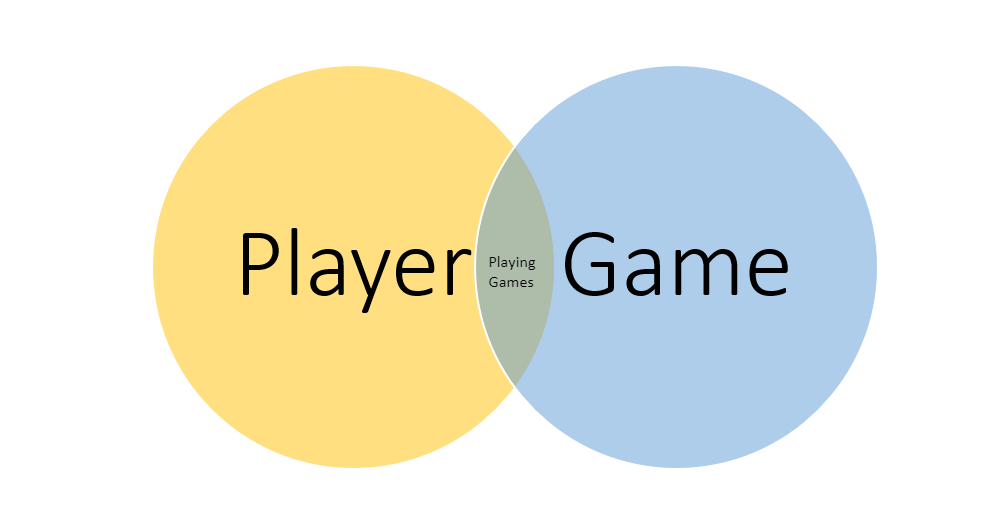
\includegraphics[width=0.75\textwidth]{figurer/PlayerAndGames.PNG}}
\caption{Overview over how the words ``Player" and ``Game" correlates with each other.}
\medskip
\small\em
\label{fig:playerGame}
\end{figure}

\subsection{Players, Games and Playing the Game}
\label{sec:PlayersGamesAndPlayingGames}
The word \textbf{``Player"} can be used to describe a person who may manipulate others to get what they want. Example of this can be a so called "Player", which is \textit{someone who manipulates someone's feelings to get what they want.} On the other hand in our project the ``Player" we describes is the person who simply playes a game.\cite[P.~19-20]{RealityIsBroken}.

The word \textbf{``Game"} often used to referred to as "Gaming", but can be used as the expression \textit{``Gaming the system"} which means something entirely different. \textit{it means that you are exploiting the system for your own personal gain.} This is simply not the definition we are looking for. In this case it is the product that the ``Player" will use, an interactive media.\cite[P.~19-20]{RealityIsBroken}.

When is coming to \textbf{``Playing the Game"} which is the act we get from combining these words, the first we think of someone who plays a video games and such. For others this can be interpretation as \textit{someone who potentially manipulate someone to break their own morals or ethics.}\cite[P.~19-20]{RealityIsBroken}. 

This is probably some of the many reasons that some people have issues with players. They don't trust them, they keep their guards up and can we really blame them for that? They might be afraid that someone will use strategy to manipulate them for their own personal gain, or amusement. They don't want to be played with. Like when someone says "We are not playing a game". They want the person to stop acting foolish and recklessly, and start to take things seriously. This is a big part of the reason why some think that games trains us to act a way that aren't appropriate for ``real-life". Like when some say that violent games like ``shooting games" are the reason why some people are violent. That the are the games that makes people violent and nothing else. All of these metaphor's does not reflect what it means to play a well-designed game. These metaphor's just are a reflection of their own worst fear, and the fear lies in keeping track of where the game begin and where it really ends. To fix how games are viewed we need to focus on how real games works and how to act and interact when we are playing them, either if it is alone or with others.\cite[P.~19-20]{RealityIsBroken}. 

\subsection{What is a Game?}
\label{sec:WhatAGameIs}  
To find a good definition for what a game is, we need to strip it down to it's core. Like \textit{McGonigal} carefully explained is that they all shares the same four traits: \textit{a goal, rules, a system for feedback and voluntary participation}.

The \textbf{goal} is the outcome that the player will work to achieve. It gives the player something to set their focus and attention on. It motivates them and gives them a reason and a sense of purpose. The \textbf{rules} are there for a reason, to place limitations for the players. It decides among other things as how the player can achieve the goal. It can be a part of what pushes the player to explore new territories and possibilities. This will unleash the players creativity and give growth to strategic thinking. What the \textit{feedback system} does is to tell the players how close they are to achieve their goal by giving them points, levels, stats and a progress bar. It can also be as simple as letting the player know the outcome such as "Game Over" and "You Win!". You can also motivate the player in real-time to make them keep going. When it comes to \textit{voluntary participation} it requires that everyone which is participating, playing the game, knowingly and willingly accepts the goal, rules and the feedback. Knowing this is what establishes a common ground for several people to play along together. They have the freedom to leave whenever they want and this ensures that the player, that plays stressing and challenging games is experienced as safe and pleasurable.\cite[P.~20-22]{RealityIsBroken}

\subsection{Types of Game and Gameplay}
\label{sec:GameAndGaePlay}
First of all games comes inn all shape and sizes, and with that I mean platform and genre. There are games that are meant for just only one person, so called "Single-Player", and there's games meant to play with other in some kind of way either if it CO-OP, which I think just stands for \textit{Cooperative}, or Online over the World Wide Web. Another way of playing together in a big community and that's MMO \textit{``Massive Multiplayer Online"}, the different choices when it comes to where and how to game doesn't stop here. First is the standard choice, which I personally prefer, but there is also console such as "Playstation", in this generation called "PS4", "Xbox", the latest edition is called "Xbox One". Another option is handheld console, which can be even your phone, or something more "game friendly" like "Nintendo Switch". So the choice really is yours. I personally believes that there is a game for everyone.
\cite[P.~20]{RealityIsBroken}.

\subsection{Game Definition}
\label{sec:GameDefenition}
What we think of when we are asked to define a game are thing such as graphics, narrative, virtual environment, competition, rewards and interactivity. But these are only common features, especially when it comes to today's games. What actually defines it are the goals, rules, feedback and voluntarily. The other stuff is just features which enhance and may or may not reinforce the four core elements. A story can make the goal more alluring and exiting to achieve. Scoring can make the feedback system more motivating. Achievement increases the the opportunities for success, and multiplayer can make the time in the game more pleasurable and unpredictable. Graphics, sounds and 3D environment can help us sustain our attention to the work we are doing in the game. Algorithms can be used to increase difficulty, which are one of many ways to redefine the goal and introduce more challenge to the game. Bernard Suits, a philosopher defines what a game is in a simple yet understandable way. \textit{"Playing a game is the voluntary attempt to overcome unnecessary obstacles"}.\cite[P.~55]{TheGrasshopper} That definition explains everything that is fun, motivating and rewarding about playing games. So we may think of games as an invitation to go and tackle a bunch of unnecessary obstacles.\cite[P.22]{RealityIsBroken} 

\subsection{Why do we play Games?}
\label{WhyWePlay}
\textbf{``Gamers"} as we call them are those who wants to play the games, they want to learn and explore, and improve themselves. They are volunteering for this unnecessary hard work and they care deeply about the outcome of their effort. That the thing, nothing really makes us happier than honest hard work. Games may be more important then we first thought, if we listen to the words of psychologist Brian Sutton-Smith we might get a deeper sense of why we play games as much as we do. \textit{"The opposite of play, in these terms, is not a present reality or work, it is vacillation, or worse, it is depression."}\cite[P.~198]{AmbiguityOfPlay}. According to this definition, we humans suffers from two things: \textit{``A pessimistic sense of inadequacy and a despondent lack of activity."}\cite{depressionwebsite}. This is the definition of depression itself. The opposite of this will be: \textit{"An optimistic sense of our own capabilities and an invigorating rash of activity."} \cite[P.~28]{RealityIsBroken}. This is an ideal description of the emotional state of gameplay, this is the exact opposite of the definition to Brian Sutton-Smith and that means that gameplay in other words is the emotional opposite of depression. If you think about it, games gives us the opportunity to focus our energy on something that is enjoyable and we're good at. If only that hard work applied in the real world, but that may be because that often is something we has to do. This could either be to make a living, to just meet someone's expectation of us, or just because someone else gave us a job to do. That is something we recent, it stresses us  and take time away time from family and friends. These jobs often comes with criticism, we're afraid of failing and we don't see the result of our effort which is disappointing and leaves us not with the feeling of satisfaction.This is precisely what the game industry does, it's fulfilling our need and gives us the hard work that we enjoy and care about. \cite[P.~28-36]{RealityIsBroken}.

\section{Theoretical Foundation}
\label{sec:Reasearch} The idea of making something that is unique and original is quite exciting in it self, it took a lot of effort and unfortunately time to create the concept behind it. We had to do a lot of research for designing the concept art, the gameplay, the core mechanics, animation and the story behind it all. The environment is a big part of setting the mood for the game. For the concept artists was it important to establish the environment and the feel of the game. The character design were quite important to figure out early on, because they will get a lot of attention, especially the main character which is the one the player uses to interact with the game. There is a long process when designing characters, but that will be discussed further later on. The technology behind it all where really time consuming to set up, like the combat system. This was somewhat complicated to set up, along with the shop and inventory system. In addition to this we had to find some ambient music to set the player in the right state of mind. If we use the wrong type of music, it might give the user the wrong idea and make them confused. So just to sum it up, it required a lot of research to make this game.


\subsection{Goal and Target Group}
\label{sec:GoalAndTarget}
The development team behind "CardLords High School", consists of six members in their early twenties, which lead us to choose teens and young adults for the target group. That gave us an advantage, because then we are a part of the target audience our self. Developing a game for a much younger or older audience, would have demanded a lot more research and taken a lot more time deciding on what the project should be.    
The target audience will not be suitable for the younger part of the population because of some harsh language and displaying of violence and drugs. It's recommended that the users of this product would be 16 or older.

\newpage
\subsection{Technology}
\label{sec:Reasearch}
For this project we are using a set of different kind of tools. The programs we have taken usage of is:
\begin{itemize} 
\item \textbf{Game engine:} Unreal Engine 4.24.2(UE4)
\item \textbf{Coding IDE:} Visual Studio 2019, this is used for coding along with the Unreal engine.
\item \textbf{Cooperation platform:} GitHub Desktop, this is used for working on the project alongside each other and has been crucial in the process of cooperation alongside programmers and artists.
\item \textbf{Communication platform:} Discord and on some occasions Zoom, this is a way for us to communicate with each other without being in the same room.
\item \textbf{Modeling and animation:} Autodesk Maya 2018, this has been used to create assets and animate the characters.
\item \textbf{Painted textures:} Krita, used to make the hand painted textures.
\item \textbf{Drawing and texturing:} Clip StudioPaint, Paintstorm Studios and Paint Tool Sai, used by the concept artists for character design.
%Any Other programs
\end{itemize}
%TEXT
